\section{\content{注音符號、漢語拼音簡介}{汉语拼音、注音符号简介}}\label{section:bopomofo-pinyin}
\subsection{\content{背景知識}{背景知识}}
\content{回想一下,在你幼時初學漢語(如果你的母語是漢語)的過程中,你是否有過「能認得某個字,但就是不會寫」的經歷?你也可以問問身邊常用漢語的朋友們,他們是否常常提筆忘字?}{回想一下,在你幼时学习汉语(如果你的母语是汉语)的过程中,你是否有过“能认得某个字,但就是不会写”的经历?你也可以问问身边常用汉语的朋友们,他们是否常常提笔忘字?}\par
\content{這樣的情況並不鮮見,因為語言習得的正常規律是從「聽」和「說」開始的。當我們開始學寫字時,其實我們早就會唸不少字了;每學一個新字時,我們也總會更關注它的讀音,而不是寫法。}{这样的情况并不鲜见,因为语言习得的正常规律是从“听”和“说”开始的。当我们开始学写字时,其实我们早就会念不少字了;每学一个新字时,我们也总会更关注它的读音,而不是写法。}\par
\content{我們判斷自己是否「認識」某個字,往往也要以「是否會唸」作為依據。舉些例子,「\textbf{柃}木」「\textbf{囿}於」「虎\textbf{兕}」「\textbf{朊}粒」「\textbf{旻}天」中的五個粗體字,簡單到只要让人看過一眼就會寫了,但是你真的認得它們嗎?與之相反,對於「食\textbf{鹽}」「\textbf{黎}明」「\textbf{罐}頭」「\textbf{贏}家」中的四个粗體字,我們未必都會寫(或許正是人們提筆忘字的範例),但是我們只要看上一眼就可以確信,我們認識這些字!}{我们判断自己是否“认识”某个字,往往也要以“是否会念”作为依据。举些例子,“\textbf{柃}木”“\textbf{囿}于”“虎\textbf{兕}”“\textbf{朊}粒”“\textbf{旻}天”中的五个粗体字,简单到只要让人看过一眼就会写了,但是你真的认得它们吗?与之相反,对于“扫\textbf{帚}”“\textbf{黎}明”“\textbf{罐}头”“\textbf{赢}家”中的四个粗体字,我们未必都会写(或许正是人们提笔忘字的范例),但是我们只要看上一眼就可以确信,我们认识这些字!}\par
\content{可見,我們對「字音」的印象要比對「字形」深得多,所以在學習任何字時,掌握其讀音都是很有必要的。就書面注音而言,現代人一般使用注音符號或漢語拼音來為漢字注音,而古人則使用反切等方法為漢字注音。本節將對漢語注音方法的發展做簡要介紹。}{可见,我们对“字音”的印象要比对“字形”深得多,所以在学习任何字时,掌握其读音都是很有必要的。就书面注音而言,现代人一般使用汉语拼音或注音符号来为汉字注音,而古人则使用反切等方法为汉字注音。本节将对汉语注音方法的发展做简要介绍。}\par
\subsubsection{\content{同音相注法}{同音相注法}}
\content{試想,如果不能用注音/拼音這樣的記號,我們要怎麼表示一個字的讀音呢?最簡單的方法就是用另一個讀音相同的字來為它注音,這就是同音相注法,或稱直音法。}{试想,如果不能用拼音/注音这样的记号,我们要怎么表示一个字的读音呢?最简单的方法就是用另一个读音相同的字来为它注音,这就是同音相注法,或称直音法。}\par
\begin{wrapfigure}{O}{.5\textwidth}
    \centering
    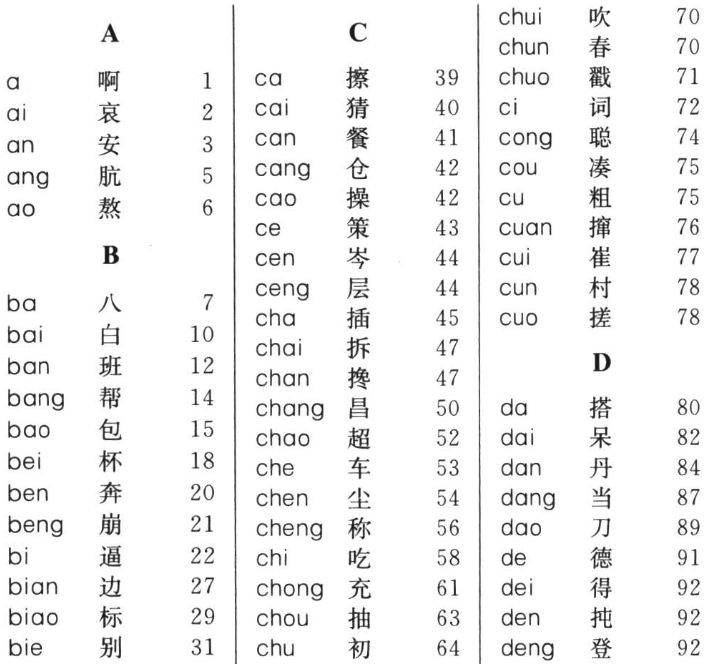
\includegraphics[width=.5\textwidth]{新華字典中的同音相注法.png}
    \caption{\content{新華字典中的音節索引}{新华字典中的音节索引}}
    \label{figure:新華字典中的同音相注法}
    {\footnotesize\color{darkgray} \content{索引中保留了同音相注法}{索引中保留了同音相注法}}
\end{wrapfigure}
\content{舉個簡單的例子,如果要為「庵」字注音,我們可以用「安」字。這樣一來,稍有讀音知識的人都可以透過「安」字得知「庵」字的讀音。}{举个简单的例子,如果要为“庵”字注音,我们可以用“安”字。这样一来,稍有读音知识的人都可以通过“安”字得知“庵”字的读音。}\par
\content{《新華字典》的音節索引頁中既有拼音,又有對應拼音的例字(\cref*{figure:新華字典中的同音相注法})。我們可以認為這是某種意義上的「同音相注」:比如,與「安」同音的字在第三頁。}{《新华字典》的音节索引页中既有拼音,又有对应拼音的例字(\cref*{figure:新華字典中的同音相注法})。我们可以认为这是某种意义上的“同音相注”:比如,与“安”同音的字在第三页。}\par
\content{但是,同音相注法的缺陷也是顯而易見的:如果一個人連常用的漢字都認不全,那他就很難透過已有的讀音知識來判斷新漢字的讀音了。}{但是,同音相注法的缺陷也是显而易见的:如果一个人连常用的汉字都认不全,那他就很难通过已有的读音知识来判断新汉字的读音了。}\par
\content{同音相注法還有其它的尷尬之處。仍以\cref*{figure:新華字典中的同音相注法}為例,我們看「岑」字,這並不是一個常用字,很多人不認得它。然而,同讀音(\pinyin{cen}\ ㄘㄣ)之下已沒有更常用的字,我們要想同音相注的話,根本找不到合適的選擇!}{同音相注法还有其它的尴尬之处。仍以\cref*{figure:新華字典中的同音相注法}为例,我们看“岑”字,这并不是一个常用字,很多人也不认得它。然而,同读音(\pinyin{cen}\ ㄘㄣ)之下已没有更常用的字,我们要想同音相注的话,根本找不到合适的选择!}\par
\subsubsection{反切法}
\content{反\textbf{切}\textsuperscript{千介切}法在古漢語注音系統中有著舉足輕重的地位。它的基本思路是「二字注一字」:取第一字(上字)的聲母和第二字(下字)的韻母及音調\footnote{這樣說不太準確。關於音調,準確的說法是「陰陽判於上字,平仄斷乎下字」,即上下二字共同決定音調。然而,古今音調規則相差很大,本書無意在此處細究,故正文不提。},拼合起來就是所求之字(歸字)的讀音。}{反\textbf{切}\textsuperscript{千介切}法在古汉语注音系统中有着举足轻重的地位。它的基本思路是“二字注一字”:取第一字(上字)的声母和第二字(下字)的韵母及音调\footnote{这样说不太准确。关于音调,准确的说法是“阴阳判于上字,平仄断乎下字”,即上下二字共同决定音调。然而,古今音调规则相差很大,本书无意在此处细究,故正文不提。},拼合起来就是所求之字(归字)的读音。}\par
\begin{wrapfigure}{O}{.4\textwidth}
    \centering
    \vspace{-2em}
    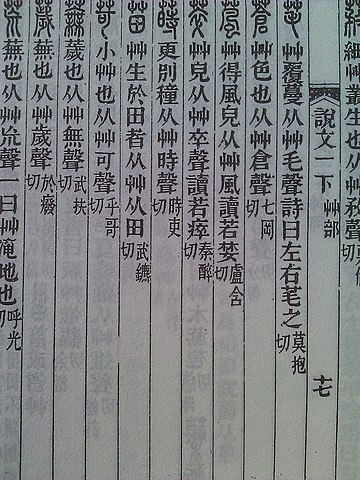
\includegraphics[width=.4\textwidth]{說文-艸部.jpeg}
    \caption{\content{大徐本《說文》草部}{大徐本《说文》草部}}
    \label{figure:說文-艸部}
    {\footnotesize\color{darkgray}\content{圖片來源:維基共享資源}{图片来源:维基共享资源}}
\end{wrapfigure}
\content{方才文中標粗的「切」字是用「千」「介」二字來注音的,我們在拼讀「切」字時,只需取上字「千」的聲母「\pinyin{q}\ ㄑ」和下字「介」的韻調「\pinyin{ie4}\ ㄧㄝˋ」就可以拼出「切」的字音「\pinyin{qie4}\ ㄑㄧㄝˋ」了。}{方才文中标粗的“切”字是用“千”“介”二字来注音的,我们在拼读“切”字时,只需取上字“千”的声母“\pinyin{q}\ ㄑ”和下字“介”的韵调“\pinyin{ie4}\ ㄧㄝˋ”就可以拼出“切”的字音“\pinyin{qie4}\ ㄑㄧㄝˋ”了。}\par
\content{反切注音比同音相注靈活得多,比如「岑」字可以用「才」「人」二字切出,這樣就能在一定程度上避免同音相注法「無字可注」的尷尬。}{反切注音法比同音相注灵活得多,比如“岑”字可以用“才”“人”二字切出,这样就能在一定程度上避免同音相注法“无字可注”的尴尬。}\par
\content{更重要的是,反切對於語音系統的分析更為透徹。從反切開始,人們已經有了完善的聲韻觀念和系統化的拼讀規則。一個人只需認得一些常見的反切上下字,就可以拼讀任何注音文字。東漢以後,反切法大行其道,無論韻書、辭典,無一不用反切注音(\cref*{figure:說文-艸部})。}{更重要的是,反切对于语音系统的分析更为透彻。从反切开始,人们已经有了完善的声韵观念和系统化的拼读规则。一个人只需认得一些常见的反切上下字,就可以拼读任何注音文字。东汉以后,反切法大行其道,无论韵书、辞典,无一不用反切注音(\cref*{figure:說文-艸部})。}\par
\subsubsection{\content{威妥瑪拼音}{威妥玛拼音}(Wei\textsuperscript{1}\ T'o\textsuperscript{3}-ma\textsuperscript{3}\ P'in\textsuperscript{1}-yin\textsuperscript{1})}
\content{威妥瑪拼音產生於19世紀後半葉,它是使用拉丁字母為漢語注音的較早嘗試,也是19\textasciitilde20世紀期間使用最為廣泛的拉丁注音。}{威妥玛拼音产生于19世纪后半叶,它是使用拉丁字母为汉语注音的较早尝试,也是19\textasciitilde20世纪期间使用最为广泛的拉丁注音。}\par
\content{在漢語拼音出現後,威妥瑪拼音已經逐漸被漢語拼音所取代。但是,我們仍然可以在部分英譯名中看到威妥瑪拼音的痕跡,比如「北京大學」是「\textbf{Peking} University」,「台北」是「\textbf{Taipei}」,「太極」是「\textbf{Taichi}」,「易經」是「{\bf I Ching}」。這些都是威妥瑪拼音的拼法。}{在汉语拼音出现后,威妥玛拼音已经逐渐被汉语拼音所取代。但是,我们仍然可以在部分英译名中看到威妥玛拼音的痕迹,比如“北京大学”是“\textbf{Peking} University”,“台北”是“\textbf{Taipei}”,“太极”是“\textbf{Taichi}”,“易经”是“{\bf I Ching}”。这些都是威妥玛拼音的拼法。}\par
\content{威妥瑪拼音是用來拼讀現代標準漢語的,它與注音符號、漢語拼音之間有較好的對應關係。威妥瑪拼音的使用時間相當長,直到2008年,台灣在仍廣泛使用。}{威妥玛拼音是用来拼读现代标准汉语的,它与注间符号、汉语拼音之间有较好的对应关系。威妥玛拼音的使用时间相当长,直到2008年,台湾仍在广泛使用。}\par
\begin{wrapfigure}{I}{.4\textwidth}
    \centering
    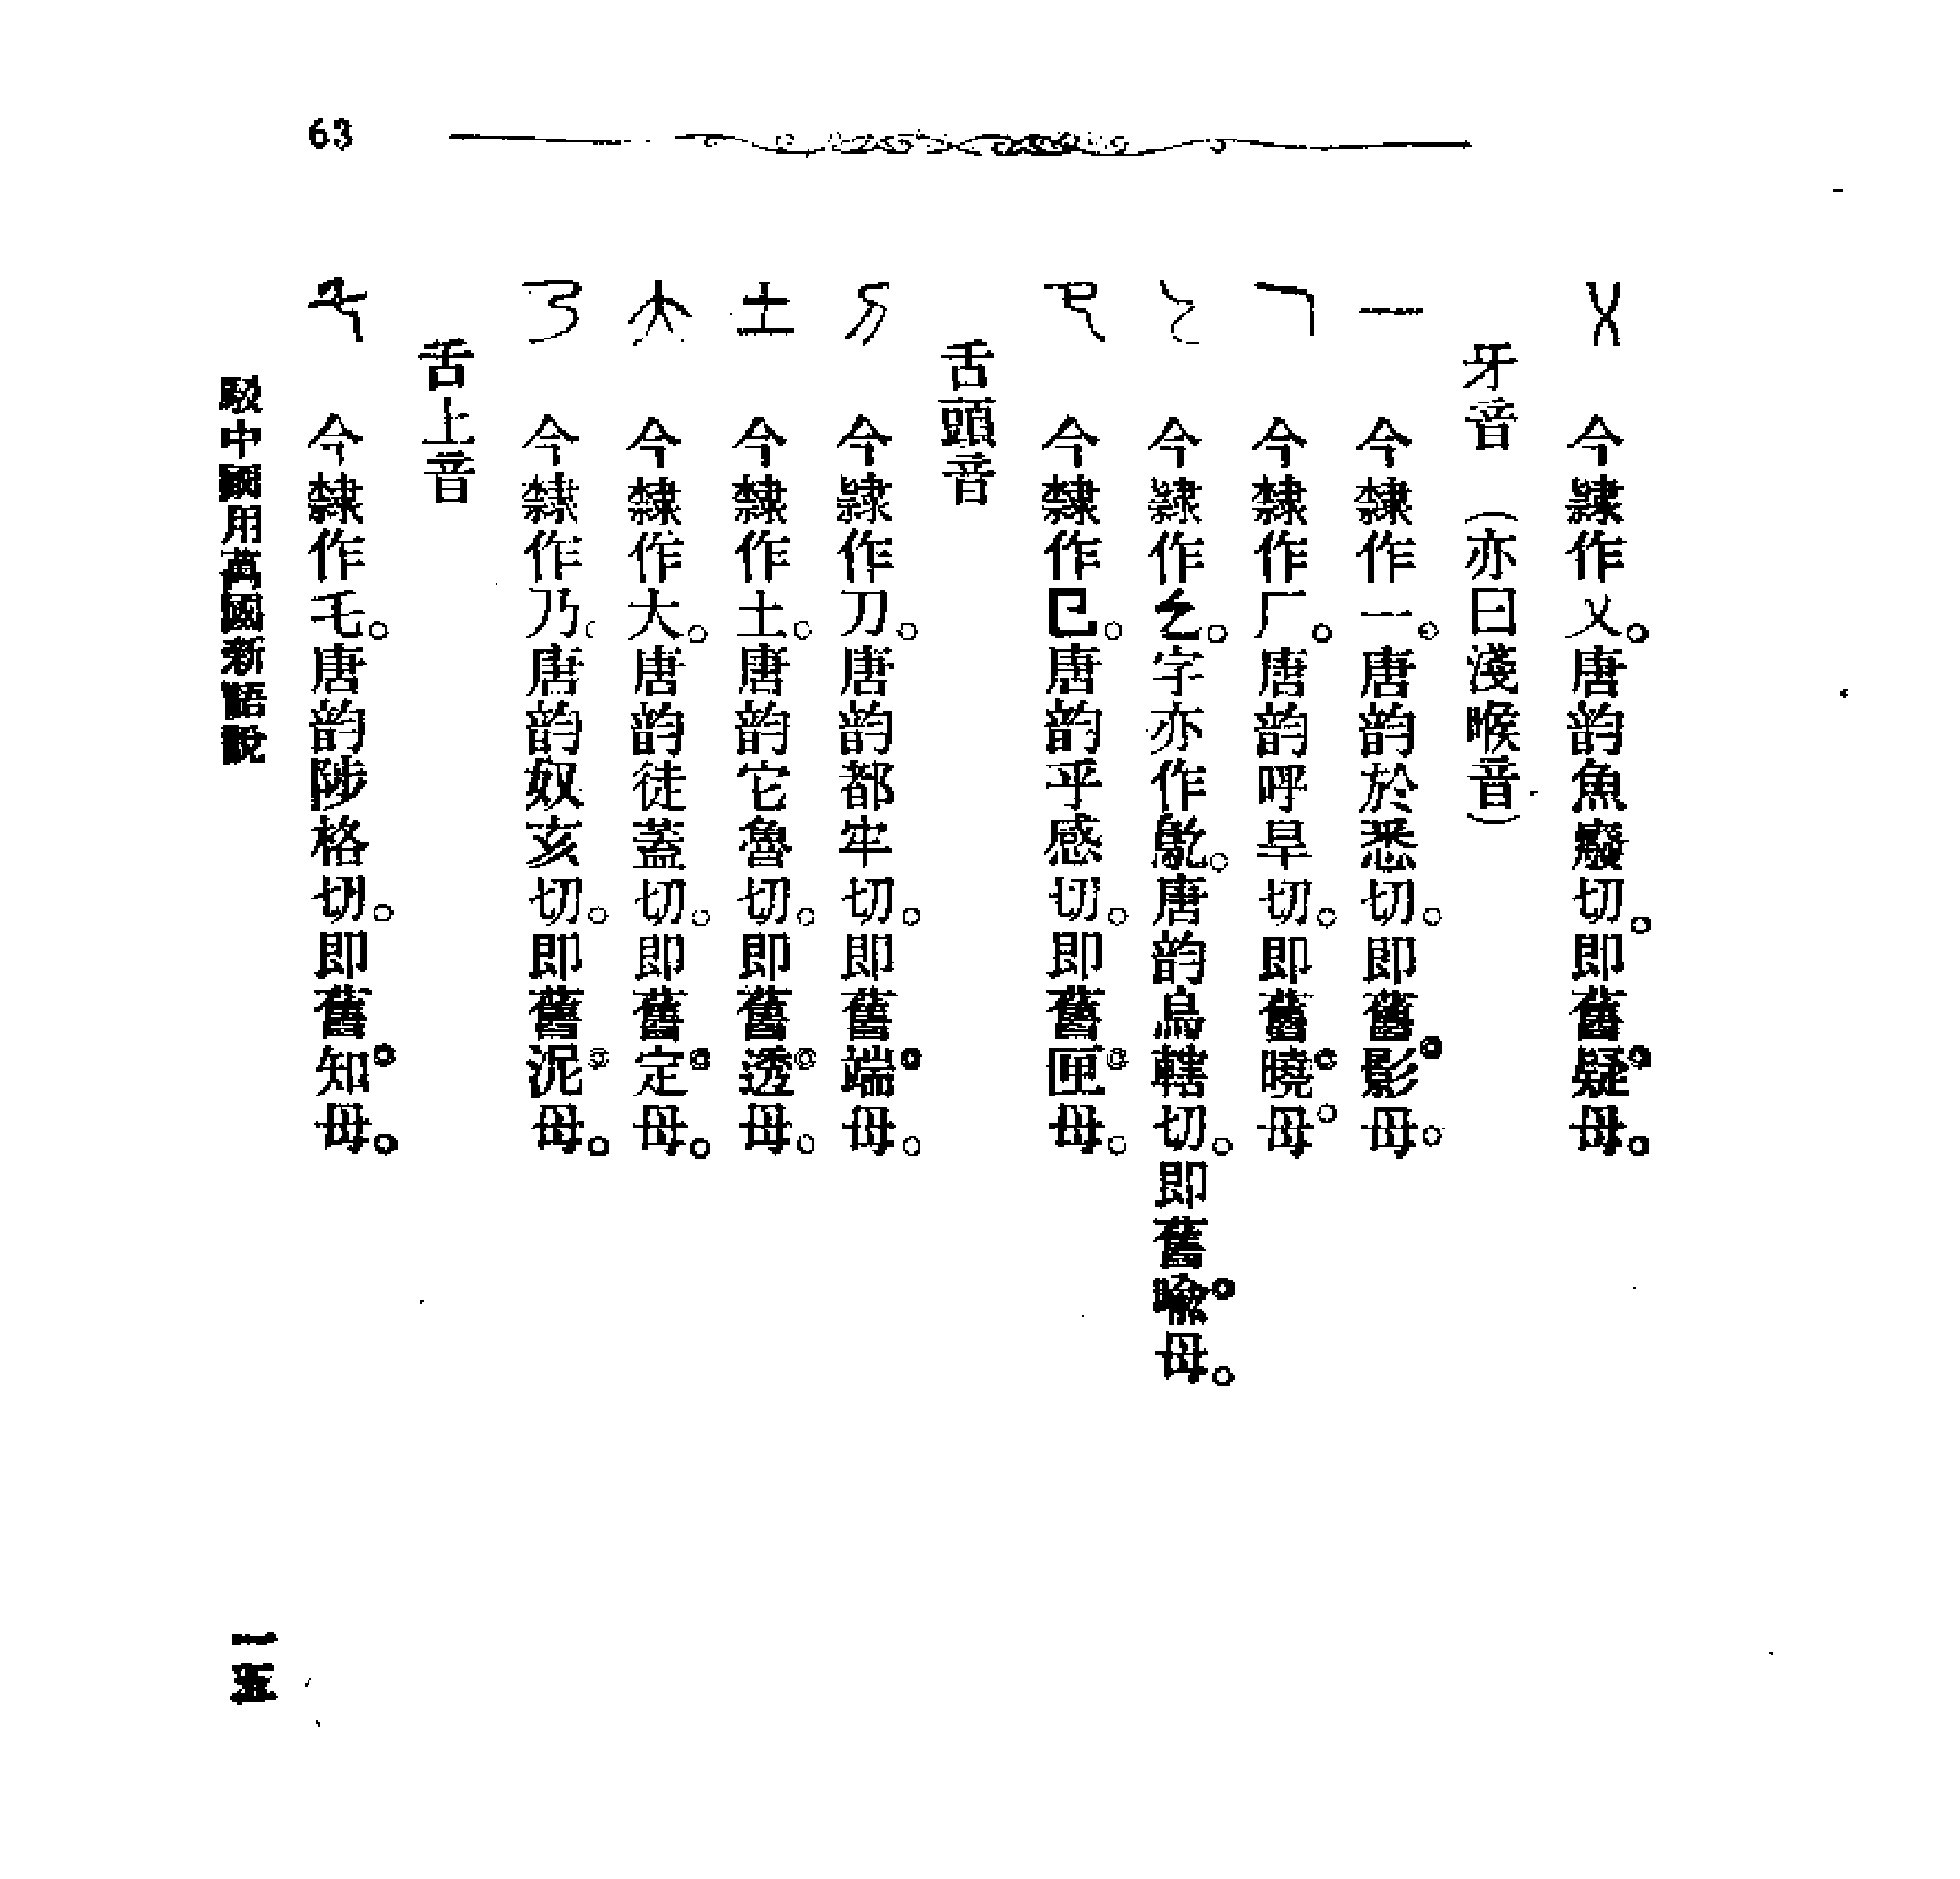
\includegraphics[width=.4\textwidth]{章太炎《駁中國用萬國新語說》「紐文」一頁.png}
    \caption{\content{章太炎《駁中國用萬國新語說》中的一頁,介紹的是紐文}{章太炎《驳中国用万国新语说》中的一页,介绍的是纽文}}
    \label{figure:章太炎《駁中國用萬國新語說》「紐文」一頁}
    {\footnotesize\color{darkgray}\content{《民報》第21號}{《民报》第21号}}
\end{wrapfigure}
\parbox[-1em]{0em}{}
\vspace{-2em}
\subsubsection{\content{注音符號}{注音符号}(ㄓㄨˋㄧㄣㄈㄨˊㄏㄠˋ)}
\content{回顧一下前面講到的反切法吧。它的思路是很清晰的:一「聲」一「韻」得一字。但在實際操作中,反切法是用另兩個字分別提供的聲母和韻母來為某個字注音的。按維基大典的說法\footnote{\href{https://zh-classical.wikipedia.org/wiki/反切\#圓缺}{反切\#圓缺 - 維基大典}},反切法需要約四百個上字,約一千個下字,這就要求反切法的使用者先得認識許多字的讀音。而在使用反切法的過程中,我們還需要把上字的聲和下字的韻調分別提取出來再拼合,這個過程也是十分繁瑣的。}{回顾一下前面讲到的反切法吧。它的思路是很清晰的:一“声”一“韵”得一字。但在实际操作中,反切法是用另两个字分别提供的声母和韵母来为某个字注音的。按维基大典的说法\footnote{\href{https://zh-classical.wikipedia.org/wiki/反切\#圓缺}{反切\#圓缺 - 維基大典}},反切法需要约四百个上字,约一千个下字,这就要求反切法的使用者先得认识许多字的读音。而在使用反切法的过程中,我们还需要把上字的声和下字的韵调分别提取出来再拼合,这个过程也是十分繁琐的。}\par
\content{如果我們要重新設計一套拼讀系統的話,自然不難想到,其實我們完全可以自訂一套聲母和韻母,根本沒必要用別的漢字來「反切」聲韻。這也正是清末許多學者努力的方向。}{如果我们要重新设计一套拼读系统的话,自然不难想到,其实我们完全可以自定义一套声母和韵母,根本没必要用别的汉字来“反切”声韵。这也正是清末许多学者努力的方向。}\par
\content{章太炎模仿日語假名的做法,借用漢字的偏旁等部件創造了若干「紐文」「韻文」,這是注音符號的前身(\cref*{figure:章太炎《駁中國用萬國新語說》「紐文」一頁})。中華民國教育部在章太炎所創方案的基礎上制訂了初代「注音字母」。其後,這套方案又經過歷次修改,終於形成了我們現在看到的「注音符號」。}{章太炎模仿日语假名的做法,借用汉字的偏旁等部件创造了若干“纽文”“韵文”,这是注音符号的前身(\cref*{figure:章太炎《駁中國用萬國新語說》「紐文」一頁})。中华民国教育部在章太炎所创方案的基础止制定了初代“注音字母”。其后,这套方案又经过历次修改,终于形成了我们现在看到的“注音符号”。}\par
\content{現今,注音符號在台灣廣泛使用,也是台灣小學生的必修課。而在中國大陸、香港和澳門,注音符號的使用相對較少。}{现今,注音符号在台湾广泛使用,也是台湾小学生的必修课。而在中国大陆、香港和澳门,注音符号的使用相对较少。}\par
\subsubsection{\xpinyin*{\content{漢語拼音}{汉语拼音}}}
\content{如果說注音符號是「假名派」,仿用假名的思路創造聲符;那麼漢語拼音和威妥瑪拼音一樣,都屬於「拉丁派」,使用拉丁字母來創造聲符。}{如果说注音符号是“假名派”,仿用假名的思路创造声符;那么汉语拼音和威妥玛拼音一样,都属于“拉丁派”,使用拉丁字母来创造声符。}\par
\content{漢語拼音系統始於1950年代,是由王力等語言學家整合早期漢字拉丁化基礎與各種拼音方案而開發出的新拼音方案。相比於威妥瑪拼音等舊方案,漢語拼音易於學習和使用(尤其是節省了許多修飾符),無論手寫還是電腦輸入都十分方便。}{汉语拼音系统始于1950年代,是由五力等语言学家整合早期汉字拉丁化基础与各种拼音方案而开发出的新拼音方案。相比于威妥玛拼音等旧方案,汉语拼音易于学习和使用(尤其是省略了许多修饰符),无论手写还是电脑输入都十分方便。}\par
\content{現今,漢語拼音方案已經成为漢字轉寫為拉丁字母的規範方式,也是國際普遍承認的漢語拉丁轉寫標準。中國大陸和香港、澳門都將漢語拼音作為小學生的必修課;台灣於2008年起开始採用漢語拼音替代威妥瑪拼音和通用拼音\footnote{通用拼音是台灣的本土拉丁字母拼音方案,於2002年推行,但不久後就被漢語拼音所替代。}。}{现今,汉语拼音方案已经成为汉字转写为拉丁字母的规范方式,也是国际普遍承认的汉语拉丁转写标准。中国大陆和香港、澳门都将汉语拼音作为小学生的必修课;台湾于2008年起开始采用汉语拼音替代威妥玛拼音和通用拼音\footnote{通用拼音是台湾的本土拉丁字母拼音方案,于2002年推行,但不久后就被汉语拼音所替代。}。}\par
\subsection{\content{由漢語拼音推導注音符號}{由汉语拼音推导注音符号}}
\subsubsection{\content{注音符號的記憶}{注音符号的记忆}}
\content{注音符號與漢語拼音之間存在很好的對應關係,所以要把一者「翻譯」成另一者是非常簡單的。對於掌握漢語拼音而初學注音符號的人來說,最大的困難其實是——辨認這些符號並記憶它們的讀音還滿不容易的。}{注音符号与汉语拼音之间存在很好的对应关系,所以要把一者“翻译”成另一者是非常简单的。对于掌握汉语拼音而初学注音符号的人来说,最大的因难其实是——辨认这些符号并记忆它们的读音还是挺不容易的。}\par
\content{筆者認為,了解注音符號的「字源」並與已有的漢字知識建立適當的聯係,是快速掌握注音符號的不二法門。注音符號雖為人造,但也有章法可循,多以古字、異體字或其部件構成,取其聲、韻而得。因此,哪怕只是簡單了解其字源,都可能對學習注音符號大有禆益——至少,有很多符號不需要靠死記硬背來記憶了。}{笔者认为,了解注音符号的“字源”并与已有的汉字知识建立适当的联系,是快速掌握注音符号的不二法门。注音符号虽为人造,但也有音法可循,多以古字、异体字或其部件构成,取其声、韵而得。因此,哪怕只是间单了解其字源,者可能对学习注音符号大有禆益——至少,有很多符号不需要靠死记硬背来记忆了。}\par
\content{\href{https://zh.wikipedia.org/zh-tw/注音符號\#符號字源及發音}{注音符號\#符號字源及發音 - 維基百科}為我們提供了一份詳盡的列表,可供讀者考查字源。}{\href{https://zh.wikipedia.org/zh-cn/注音符號\#符號字源及發音}{注音符号\#符号字源及发音 - 维基百科}为我们提供了一份详尽的列表,可供读者考查字源。}\par
\content{\cref{appendix:注音符號、漢語拼音表}是筆者根據維基百科及《漢語拼音方案》等資料整理而成的,可以作為注音、拼音轉換的可靠參考。}{\cref{appendix:注音符號、漢語拼音表}是笔者根据维基百科及《汉语拼音方案》等资料整理而成的,可以作为注音、拼音转换的可靠参考。}\par
\content{但是,筆者並不很喜歡這個表格。它看上去很轉業,也很詳盡,但它的韻母表太過複雜,容易讓讀者望而卻步。筆者更喜歡用「推導」替代「記憶」,即,只需要記住\textbf{必備的基礎}和\textbf{推導的規則},然後把剩下的部分交給推導而非記憶。我們在學習繁簡轉換的過程中將常常與這種方法打交道,比如,若是你知道「馬」的簡化字是「马」,那麼猜想「媽」的簡化字是「妈」就滿合理的。}{但是,笔者并不很喜欢这个表格。它看上去很专业,也很详尽,但它的韵母表太过复杂,容易让读者望而却步。笔者更喜欢用“推导”替代“记忆”,即,只需要记住\textbf{必备的基础}和\textbf{推导的规则},然后把剩下的部分交给推导而非记忆。我们在学习繁简转换的过程中将常常与这种方法钉交道,比如,若是你知道“马”的繁体字是“馬”,那么猜想“妈”的繁体字是“媽”就蛮合理的。}\par
\subsubsection{\content{必備的基礎}{必备的基础}}
\content{筆者最初是透過注音鍵盤來接觸注音的。\cref*{figure:大千式注音鍵盤}展示了一種常見的注音鍵盤——大千式注音鍵盤。它把21個聲母、3個介母\footnote{介母是韻母的一種。在注音符號系統中,介母從韻母中單列出來——我們將在後文中看到,這種做法是有意義的;而在漢語拼音等方案中,明確區分出「介母」的概念已無必要。}和13個韻母從左到右,依次擺放起來。至於\cref{table:韻母表}中眾多的韻母,它們無非都是由這些介母和韻母組合而成的。}{笔者最初是通过注音键盘来接触注音的。\cref*{figure:大千式注音鍵盤}展示了一种常见的注音键盘——大千式注音键盘。它把21个声母、3个介母\footnote{介母是韵母的一种。在注音符号系统中,介母从韵母中单列出来——我们将在后文中看到,这种做法是有意义的;而在汉语拼音方案中,明确区分出“介母”的概念已无必要。}和13个韵母从左到右,依次摆放起来。至于\cref{table:韻母表}中众多的韵母,它们无非都是由这些介母和韵母组合而成的。}\par
\content{只要了解了這些符號並掌握其拼讀規則,我們就可以用「注音輸入法」來打字了。}{只要了解了这些符号并掌握其拼读规则,我们就可以用“注音输入法”来打字了。}\par
\begin{figure}[H]
    \newcommand{\drawkey}[4]{
        \begin{scope}[shift={#1}]
            \draw[fill=white,draw=gray,very thick](0,0)--(1,0)--(1.1,-.1)--(1.1,-1.1)--(.1,-1.1)--(0,-1)--cycle;
            \draw[fill=#2!15,draw=gray,very thick](0,0)rectangle(1,-1);
            \node[baseline] at(.7,-.3){#3};
            \node[baseline] at(.3,-.7){\sffamily\small #4};
        \end{scope}
    }
    \newcommand{\drawlegend}[3]{
        \begin{scope}[shift={#1}]
            \draw[fill=white,draw=gray,very thick](0,0)--(.5,0)--(.55,-.05)--(.55,-.55)--(.05,-.55)--(0,-.5)--cycle;
            \draw[fill=#2!15,draw=gray,very thick](0,0)rectangle(.5,-.5) node[anchor=base west]{#3};
        \end{scope}
    }
    \centering
    \begin{tikzpicture}
        \drawkey{(0,0)}{red}{ㄅ}{1}
        \drawkey{(1.2,0)}{red}{ㄉ}{2}
        \drawkey{(2.4,0)}{black}{ˇ}{3}
        \drawkey{(3.6,0)}{black}{ˋ}{4}
        \drawkey{(4.8,0)}{red}{ㄓ}{5}
        \drawkey{(6,0)}{black}{ˊ}{6}
        \drawkey{(7.2,0)}{black}{˙}{7}
        \drawkey{(8.4,0)}{blue}{ㄚ}{8}
        \drawkey{(9.6,0)}{blue}{ㄞ}{9}
        \drawkey{(10.8,0)}{blue}{ㄢ}{0}
        \drawkey{(12,0)}{blue}{ㄦ}{-}
        \drawkey{(.4,-1.2)}{red}{ㄆ}{Q}
        \drawkey{(1.6,-1.2)}{red}{ㄊ}{W}
        \drawkey{(2.8,-1.2)}{red}{ㄍ}{E}
        \drawkey{(4,-1.2)}{red}{ㄐ}{R}
        \drawkey{(5.2,-1.2)}{red}{ㄔ}{T}
        \drawkey{(6.4,-1.2)}{red}{ㄗ}{Y}
        \drawkey{(7.6,-1.2)}{green}{ㄧ}{U}
        \drawkey{(8.8,-1.2)}{blue}{ㄛ}{I}
        \drawkey{(10,-1.2)}{blue}{ㄟ}{O}
        \drawkey{(11.2,-1.2)}{blue}{ㄣ}{P}
        \drawkey{(.8,-2.4)}{red}{ㄇ}{A}
        \drawkey{(2,-2.4)}{red}{ㄋ}{S}
        \drawkey{(3.2,-2.4)}{red}{ㄎ}{D}
        \drawkey{(4.4,-2.4)}{red}{ㄑ}{F}
        \drawkey{(5.6,-2.4)}{red}{ㄕ}{G}
        \drawkey{(6.8,-2.4)}{red}{ㄘ}{H}
        \drawkey{(8,-2.4)}{green}{ㄨ}{J}
        \drawkey{(9.2,-2.4)}{blue}{ㄜ}{K}
        \drawkey{(10.4,-2.4)}{blue}{ㄠ}{L}
        \drawkey{(11.6,-2.4)}{blue}{ㄤ}{;}
        \drawkey{(1.2,-3.6)}{red}{ㄈ}{Z}
        \drawkey{(2.4,-3.6)}{red}{ㄌ}{X}
        \drawkey{(3.6,-3.6)}{red}{ㄏ}{C}
        \drawkey{(4.8,-3.6)}{red}{ㄒ}{V}
        \drawkey{(6,-3.6)}{red}{ㄖ}{B}
        \drawkey{(7.2,-3.6)}{red}{ㄙ}{N}
        \drawkey{(8.4,-3.6)}{green}{ㄩ}{M}
        \drawkey{(9.6,-3.6)}{blue}{ㄝ}{,}
        \drawkey{(10.8,-3.6)}{blue}{ㄡ}{.}
        \drawkey{(12,-3.6)}{blue}{ㄥ}{/}
        \drawlegend{(3,-5)}{red}{\content{聲母}{声母}}
        \drawlegend{(5,-5)}{green}{\content{介母}{介母}}
        \drawlegend{(7,-5)}{blue}{\content{韻母}{韵母}};
        \drawlegend{(9,-5)}{black}{\content{聲調}{声调}};
    \end{tikzpicture}
    \caption{\content{大千式注音輪入法的鍵盤排列}{大千式注音输入法的键盘排列}}
    \label{figure:大千式注音鍵盤}
\end{figure}
\content{注音的聲母與拼音一一對應(唯有拼音中的 i u 是例外),所以我就按照注音鍵盤的順序,列出\cref*{table:注音鍵盤聲母表},以供讀者參考。}{注音的声母与拼音一一对应(唯有拼音中的 i u 是例外),所以我就按照注音键盘的顺序,列出\cref*{table:注音鍵盤聲母表},以供读者参考。}\par
\begin{table}[H]
    \centering
    \caption{\content{注音鍵盤聲母表}{注音键盘声母表}}
    \label{table:注音鍵盤聲母表}
    \vspace{.5em}
    \begin{NiceTabular}{*{6}{c}}[vlines]
        \hline
        ㄅ b & ㄉ d & & & ㄓ zh & \\
        ㄆ p & ㄊ t & ㄍ g & ㄐ j & ㄔ ch & ㄗ z \\
        ㄇ m & ㄋ n & ㄎ k & ㄑ q & ㄕ sh & ㄘ c \\
        ㄈ f & ㄌ l & ㄏ h & ㄒ x & ㄖ r & ㄙ s \\\hline
    \end{NiceTabular}
\end{table}
\content{若是縱向閱讀,你或許會發現這些符號的擺放順序很像國小時學習的「ㄅㄆㄇㄈ」「ㄉㄊㄋㄌ」「ㄍㄎㄏ」……的口訣——其實這就是方便使用者記憶鍵位而設定的啦。}{若是纵向阅读,你或许会发现这些符号的摆放顺序很像小学时学习的“b p m f”“d t n l”“g k h”……的口决——其实这就是方便使用者记忆键位而设置的啦。}\par
\content{注音中的介母,也稱作「韻頭」。顧名思義,它是韻母的「開頭」。以「強」字為例,它的一個讀音是「ㄑㄧㄤˊ \pinyin{qiang2}」。在拼讀過程中,我們可以把它拆作三部分:聲母「ㄑ q」、介母「ㄧ i」和韻母「ㄤ ang」(聲調為二聲)。其中「ㄧ i」的作用十分清晰。}{注音中的介母,也称作“韵头”。顾名思义,它是韵母的“开头”。以“强”字为例,它的一个读音是“ㄑㄧㄤˊ \pinyin{qiang2}”。在拼读过程中,我们可以把它拆作三部分:声母“ㄑ q”、介母“ㄧ i”和韵母“ㄤ ang”(声调为二声)。其中「ㄧ i」的作用十分清晰。}\par
\content{介母最有趣的地方在於,當遇到零聲母\footnote{有些音沒有聲母,比如「安」字唸作「ㄢ an」,這就是零聲母。}的情況時,作為「韻頭」的介母可以「退化」成聲母,與「韻身」組合成一個音。簡單說,\textbf{這時候「介母」的作用是聲母!}}{介母最有趣的地方在于,当遇到零声母\footnote{有些音没有声母,比如“安”字念作“ㄢ an”,这就是零声母。}的情况时,作为“韵头”的介母可以“退化”成声母,与“韵身”组合成一个音。简单说,\textbf{这时候“介母”的作用是声母!}}\par
\content{既然介母既可以做韻母,又可以做聲母,那麼注音介母與拼音聲、韻母之間的對照關係也要分成兩種情況來考慮,如\cref*{table:注音鍵盤介母表}所示。}{既然介母既可以做韵母,又可以做声母,那么注音介母与拼音声、韵母的对照关系也要分成两种情况来考虑,如\cref*{table:注音鍵盤介母表}所示。}\par
\begin{table}[H]
    \centering
    \caption{\content{注音鍵盤介母表}{注音键盘介母表}}
    \label{table:注音鍵盤介母表}
    \vspace{.5em}
    \begin{NiceTabular}{*{3}{c}}[hlines]
        \toprule
        \rowcolor{gray!50}
        注音符號 & 作韻母的拼音 & 作聲母的拼音 \\\midrule[.6pt]
        ㄧ & i & y \\
        ㄨ & u & w \\
        ㄩ & \"u & \\\bottomrule
    \end{NiceTabular}
\end{table}
\content{注音符號的韻母比拼音的韻母要「少」很多。比如拼音中的「en in un \"un」其實都是由「ㄣ en」與不同介母組合而成的:}{注音符号的韵母比拼音的韵母要“少”很多。比如拼音中的“en in un \"un”其实都是由"ㄣ en"与不同介母组合而成的:}
\begin{table}[H]
    \centering
    \vspace{.5em}
    \begin{NiceTabular}{*{4}{c}}[hlines]
        \toprule
        \rowcolor{gray!50}
        \content{無介音}{无介音} & 介音 i ㄧ & 介音 u ㄨ & 介音 \"u ㄩ \\\midrule[.6pt]
        ㄣ en & ㄧㄣ in & ㄨㄣ un & ㄩㄣ \"un \\\bottomrule
    \end{NiceTabular}
\end{table}
\content{也正因如此,這「四個」韻母在新韻\footnote{參見\href{https://zh.wikipedia.org/zh-tw/中華新韻\#\nobreakspace2005年「詩詞學會」版本}{中華新韻\#2005年「詩詞學會」版本 - 維基百科}。}和通韻\footnote{參見\href{http://www.moe.gov.cn/jyb_sjzl/ziliao/A19/202111/W020211118492193544846.pdf}{語言文字規範-中華通韻\ 試行稿}。}中都是押韻的。我們從拼音中或許很難看出這一點,但在注音中這是很明顯的!}{也正因如此,这“四个”韵母在新韵\footnote{参见\href{https://zh.wikipedia.org/zh-cn/中華新韻\#\nobreakspace2005年「詩詞學會」版本}{中华新韵\#2005年“诗词学会”版本 - 维基百科}。}和通韵\footnote{参见\href{http://www.moe.gov.cn/jyb_sjzl/ziliao/A19/202111/W020211118492193544846.pdf}{语言文字规范-中华通韵\ 试行稿}。}}\par
\content{我們在注音鍵盤上看到的韻母(\cref*{table:注音鍵盤韻母表})與拼音中學到的韻母有不少差異,這是初識注音的人需要相當注意的地方。}{我们在注音键盘上看到的韵母(\cref*{table:注音鍵盤韻母表}与拼音中学到的韵母有不少差异,这是初识注音的人需要相当注意的地方。}\par
\begin{table}[H]
    \centering
    \caption{\content{注音鍵盤韻母表}{注音键盘韵母表}}
    \label{table:注音鍵盤韻母表}
    \vspace{.5em}
    \begin{NiceTabular}{*{4}{c}}[vlines]
        \hline
        ㄚ a & ㄞ ai & ㄢ an & ㄦ er \\
        ㄛ o & ㄟ ei & ㄣ en & \\
        ㄜ e & ㄠ ao & ㄤ ang & \\
        ㄝ \^e & ㄡ ou & ㄥ eng & \\
        \hline
    \end{NiceTabular}
\end{table}
\content{讀者或許會發現,\cref*{figure:大千式注音鍵盤}中還有四個符號:「ˇ\ ˊ\ ˋ\ ˙」。它們也是注音系統的成員——聲調符號。注音和拼音採用相同的聲調符號,所以我們很容易記住每個聲調意味著什麼(\cref*{table:注音聲調表})。}{读者或许会发现,\cref*{figure:大千式注音鍵盤}中还有四个符号:“ˇ\ ˊ\ ˋ\ ˙”。它们也是注音系统的成员——声调符号。注音和拼音采用相同的声调符号,所以我们很容易记信每个声调意味着什么(\cref*{table:注音聲調表})。}\par
\begin{table}[H]
    \centering
    \caption{\content{注音聲調表}{注音声调表}}
    \label{table:注音聲調表}
    \vspace{.5em}
    \begin{NiceTabular}{*{5}{c}}[hlines]
        \toprule
        \rowcolor{gray!50}
        \content{陰平(一聲)}{阴平(一声)} & \content{陽平(二聲)}{阳平(二声)} & \content{上聲(三聲)}{上声(三声)} & \content{去聲(四聲)}{去声(四声)} & \content{輕聲}{轻声} \\\midrule[.6pt]
        \content{通常不標\footnote{在注音中,不標聲調表示一聲;這和拼音中不標聲調表示輕聲的習慣有所不同。}}{通常不标\footnote{在注音中,不标声调表示一声;这和拼音中不标声调表示轻声的习惯有所不同。}} & ˊ & ˇ & ˋ & ˙ \\\bottomrule
    \end{NiceTabular}
\end{table}
\subsubsection{\content{推導的規則}{推导的规则}}
\content{對於最簡單情況來說,拼音到注音的轉換就是機械性的「聲母、韻母分別轉換」。以「法」字為例,它的拼音是「\pinyin{fa3}」,其聲母是「f」,對應注音中的「ㄈ」;韻母是「a」,對應注音中的「ㄚ」;聲調為三聲。那麼注音形式就是「ㄈㄚˇ」。}{对于最简单情况来说,拼音到注音的转换就是机械性的“声母、韵母分别转换”。以“法”字为例,它的拼音是“\pinyin{fa3}”,其声母是“f”,对应注音中的“ㄈ”;韵母是“a”,对应注音中的“ㄚ”;声调为三声。那么注音形式就是“ㄈㄚˇ”。}\par
\content{再以「車」為例,它的一個拼音是「\pinyin{che1}」,其聲母是「ch」,對應注音中的「ㄔ」;韻母是「e」,對應注音中的「ㄜ」;聲調為一聲,在注音中一聲通常無需標出。綜上所述,它的注音形式就是「ㄔㄜ」。}{再以“车”为例,它的一个拼音是“\pinyin{che1}”,其声母是“ch”,对应注音中的“ㄔ”;韵母是“e”,对应注音中的“ㄜ”;声调为一声,在注音中一声通常无需标出。综上所述,它的注音形式就是“ㄔㄜ”。}\par
\content{接下來我就著重介紹下「不能以此類推」的幾種情況。}{接下来我就着重介绍下“不能以此类推”的几种情况。}\par
\subsubsubsection{\content{空韻母}{空韵母}}
\content{在學習拼音時,我們一定接觸過一些「整體認讀」的音。以「\xpinyin*{知}」為例,如果要強行把聲母「zh」和韻母「i」拼出來,我們是拼不出「知」字的。但是,如果\textbf{只用聲母「zh」來拼讀,我們卻是可以「拼」出此字的。}}{在学习拼音时,我们一定接触过一些“整体认读”的音。以“\xpinyin*{知}”为例,如果要强行把声母“zh”和韵母“i”拼出来,我们是拼不出“知”字的。但是,如果\textbf{只用声母“zh”来拼读,我们却是可以“拼”出此字的。}}\par
\content{對於「zh ch sh r z c s」七個聲母來說,它們可以獨立成音,而不需要韻母,我們把這種情況稱作空韻母\footnote{實際上它們的韻母是「ㄭ -i」,這是一個不同於「ㄧ i」的韻母音。但「ㄭ -i」在注音系統中也一般不會使用,故正文不提。}。所以在為「知」字注音時只需要一個聲母「ㄓ」就可以了!}{对于“zh ch sh r z c s”七个声母来说,它们可以独立成音,而不需要韵母,我们把这种情况称作空韵母\footnote{实际上它们的韵母是“ㄭ -i”,这是一个不同于“ㄧ i”的韵母音。但“ㄭ -i”在注音系统中也一般不会使用,故正文不提。}。所以在为“知”字注音时只需要一个声母“ㄭ”就可以了!}\par
\content{同理,「食」「日」「思」的注音分別為「ㄕˊ」「ㄖˋ」「ㄙ」。它們都是空韻母音節。如果非要加上韻母「ㄧ」,那反而錯了。}{同理,“食”“日”“思”的注音分别为“ㄕˊ”“ㄖˋ”“ㄙ”。它们都是空韵母音节。如果非要加上韵母“ㄧ”,那反而错了。}\par
\begin{figure}[H]
    \newcommand{\drawkey}[4]{
        \begin{scope}[shift={#1}]
            \draw[fill=white,draw=gray,very thick](0,0)--(1,0)--(1.1,-.1)--(1.1,-1.1)--(.1,-1.1)--(0,-1)--cycle;
            \draw[fill=#2!15,draw=gray,very thick](0,0)rectangle(1,-1);
            \node[baseline] at(.7,-.3){#3};
            \node[baseline] at(.3,-.7){\sffamily\small #4};
        \end{scope}
    }
    \centering
    \begin{tikzpicture}
        \drawkey{(0,0)}{black}{ㄅ}{1}
        \drawkey{(1.2,0)}{black}{ㄉ}{2}
        \drawkey{(2.4,0)}{black}{ˇ}{3}
        \drawkey{(3.6,0)}{black}{ˋ}{4}
        \drawkey{(4.8,0)}{red}{ㄓ}{5}
        \drawkey{(6,0)}{black}{ˊ}{6}
        \drawkey{(7.2,0)}{black}{˙}{7}
        \drawkey{(8.4,0)}{black}{ㄚ}{8}
        \drawkey{(9.6,0)}{black}{ㄞ}{9}
        \drawkey{(10.8,0)}{black}{ㄢ}{0}
        \drawkey{(12,0)}{black}{ㄦ}{-}
        \drawkey{(.4,-1.2)}{black}{ㄆ}{Q}
        \drawkey{(1.6,-1.2)}{black}{ㄊ}{W}
        \drawkey{(2.8,-1.2)}{black}{ㄍ}{E}
        \drawkey{(4,-1.2)}{black}{ㄐ}{R}
        \drawkey{(5.2,-1.2)}{red}{ㄔ}{T}
        \drawkey{(6.4,-1.2)}{red}{ㄗ}{Y}
        \drawkey{(7.6,-1.2)}{black}{ㄧ}{U}
        \drawkey{(8.8,-1.2)}{black}{ㄛ}{I}
        \drawkey{(10,-1.2)}{black}{ㄟ}{O}
        \drawkey{(11.2,-1.2)}{black}{ㄣ}{P}
        \drawkey{(.8,-2.4)}{black}{ㄇ}{A}
        \drawkey{(2,-2.4)}{black}{ㄋ}{S}
        \drawkey{(3.2,-2.4)}{black}{ㄎ}{D}
        \drawkey{(4.4,-2.4)}{black}{ㄑ}{F}
        \drawkey{(5.6,-2.4)}{red}{ㄕ}{G}
        \drawkey{(6.8,-2.4)}{red}{ㄘ}{H}
        \drawkey{(8,-2.4)}{black}{ㄨ}{J}
        \drawkey{(9.2,-2.4)}{black}{ㄜ}{K}
        \drawkey{(10.4,-2.4)}{black}{ㄠ}{L}
        \drawkey{(11.6,-2.4)}{black}{ㄤ}{;}
        \drawkey{(1.2,-3.6)}{black}{ㄈ}{Z}
        \drawkey{(2.4,-3.6)}{black}{ㄌ}{X}
        \drawkey{(3.6,-3.6)}{black}{ㄏ}{C}
        \drawkey{(4.8,-3.6)}{black}{ㄒ}{V}
        \drawkey{(6,-3.6)}{red}{ㄖ}{B}
        \drawkey{(7.2,-3.6)}{red}{ㄙ}{N}
        \drawkey{(8.4,-3.6)}{black}{ㄩ}{M}
        \drawkey{(9.6,-3.6)}{black}{ㄝ}{,}
        \drawkey{(10.8,-3.6)}{black}{ㄡ}{.}
        \drawkey{(12,-3.6)}{black}{ㄥ}{/}
    \end{tikzpicture}
	\caption{\content{空韻母對應的注音符號在注音鍵盤中的位置}{空韵母对应的注音符号在注音键盘中的位置}}
	\label{figure:空韻母對應的注音符號在注音鍵盤中的位置}
\end{figure}
\subsubsubsection{\content{韻母推導}{韵母推导}}
\content{我們很容易看出,拼音「uai」是由介母(韻頭)「u」與韻身「ai」結合而成的。我們也不難理解,「uai」和「ai」兩個音是押韻的,它們都押在「ai」音上。}{我们很容易看出,拼音“uai”是由介母(韵头)“u”与韵身“ai”结合而成的。我们也不难理解,“uai”和“ai”两个音是押韵的,它们都押在“ai”音上。}\par
\content{但是,如果我說,「ei」和「ui」是押韻的,它們都押在「ei」音上,讀者是否會有些遲疑呢?}{但是,如果我说,“ei”和“ui”是押韵的,它们都押在“ei”音上,读者是否会有些迟疑呢?}\par
\content{其實,「ui」的完整形式應當是「uei」;只是拼音為了書寫方便之故,將其作了簡化。如果還原成「uei」,那麼我們就很容易理解它的韻腳,也很容易推導出它的注音——「u」對應「ㄨ」,「ei」對應「ㄟ」,所以「ui」就是「ㄨㄟ」啦。}{其实,“ui”的完整形式应当是“uei”;只是拼音为了书写方便之故,将其作了简化。如果还原成“uei”,那么我们就很容易理解它的韵脚,也很容易推导出它的注音——“u”对应“ㄨ”,“ei”对应“ㄟ”,所以“ui”就是“ㄨㄟ”啦。}\par
\content{類似的原理在「ㄡ ou」「ㄣ en」「ㄥ eng」中也是如此。只要我們「還原」了拼音的完整形 式,由拼音推導注音只需做一對一轉換就足矣!(\cref*{table:需要推導的韻母})}{类似的原理在“ㄡ ou”“ㄣ en”“ㄥ eng”中也是如此。只要我们“还原”了拼音的完整形式,由拼音推导注音只需做一对一转换就足矣!(\cref*{table:需要推導的韻母})}\par
\begin{table}[H]
    \centering
    \caption{需要推導的韻母}
    \label{table:需要推導的韻母}
    \vspace{.5em}
    \begin{NiceTabular}{*{4}{c}}[hlines]
        \toprule
        \rowcolor{gray!50}
        \content{所屬韻尾}{所属韵尾} & \content{標準形式}{标准形式} & \content{完整形式}{完整形式} & \content{注音符號}{注音符号} \\\midrule[.6pt]
        ㄟ ei & ui & uei & ㄨㄟ \\
        ㄡ ou & iu & iou & ㄧㄡ \\
        \Block{3-1}{ㄣ en} & in & ien & ㄧㄣ \\
        & un & uen & ㄨㄣ \\ 
        & \"un & \"uen & ㄩㄣ \\
        ㄥ eng & ing & ieng & ㄧㄣ \\\bottomrule
    \end{NiceTabular}
\end{table}
\begin{figure}[H]
    \newcommand{\drawkey}[4]{
        \begin{scope}[shift={#1}]
            \draw[fill=white,draw=gray,very thick](0,0)--(1,0)--(1.1,-.1)--(1.1,-1.1)--(.1,-1.1)--(0,-1)--cycle;
            \draw[fill=#2!15,draw=gray,very thick](0,0)rectangle(1,-1);
            \node[baseline] at(.7,-.3){#3};
            \node[baseline] at(.3,-.7){\sffamily\small #4};
        \end{scope}
    }
    \centering
    \begin{tikzpicture}
        \drawkey{(0,0)}{black}{ㄅ}{1}
        \drawkey{(1.2,0)}{black}{ㄉ}{2}
        \drawkey{(2.4,0)}{black}{ˇ}{3}
        \drawkey{(3.6,0)}{black}{ˋ}{4}
        \drawkey{(4.8,0)}{black}{ㄓ}{5}
        \drawkey{(6,0)}{black}{ˊ}{6}
        \drawkey{(7.2,0)}{black}{˙}{7}
        \drawkey{(8.4,0)}{black}{ㄚ}{8}
        \drawkey{(9.6,0)}{black}{ㄞ}{9}
        \drawkey{(10.8,0)}{black}{ㄢ}{0}
        \drawkey{(12,0)}{black}{ㄦ}{-}
        \drawkey{(.4,-1.2)}{black}{ㄆ}{Q}
        \drawkey{(1.6,-1.2)}{black}{ㄊ}{W}
        \drawkey{(2.8,-1.2)}{black}{ㄍ}{E}
        \drawkey{(4,-1.2)}{black}{ㄐ}{R}
        \drawkey{(5.2,-1.2)}{black}{ㄔ}{T}
        \drawkey{(6.4,-1.2)}{black}{ㄗ}{Y}
        \drawkey{(7.6,-1.2)}{black}{ㄧ}{U}
        \drawkey{(8.8,-1.2)}{black}{ㄛ}{I}
        \drawkey{(10,-1.2)}{blue}{ㄟ}{O}
        \drawkey{(11.2,-1.2)}{blue}{ㄣ}{P}
        \drawkey{(.8,-2.4)}{black}{ㄇ}{A}
        \drawkey{(2,-2.4)}{black}{ㄋ}{S}
        \drawkey{(3.2,-2.4)}{black}{ㄎ}{D}
        \drawkey{(4.4,-2.4)}{black}{ㄑ}{F}
        \drawkey{(5.6,-2.4)}{black}{ㄕ}{G}
        \drawkey{(6.8,-2.4)}{black}{ㄘ}{H}
        \drawkey{(8,-2.4)}{black}{ㄨ}{J}
        \drawkey{(9.2,-2.4)}{black}{ㄜ}{K}
        \drawkey{(10.4,-2.4)}{black}{ㄠ}{L}
        \drawkey{(11.6,-2.4)}{black}{ㄤ}{;}
        \drawkey{(1.2,-3.6)}{black}{ㄈ}{Z}
        \drawkey{(2.4,-3.6)}{black}{ㄌ}{X}
        \drawkey{(3.6,-3.6)}{black}{ㄏ}{C}
        \drawkey{(4.8,-3.6)}{black}{ㄒ}{V}
        \drawkey{(6,-3.6)}{black}{ㄖ}{B}
        \drawkey{(7.2,-3.6)}{black}{ㄙ}{N}
        \drawkey{(8.4,-3.6)}{black}{ㄩ}{M}
        \drawkey{(9.6,-3.6)}{black}{ㄝ}{,}
        \drawkey{(10.8,-3.6)}{blue}{ㄡ}{.}
        \drawkey{(12,-3.6)}{blue}{ㄥ}{/}
    \end{tikzpicture}
    \caption{\content{需要推導的四個韻母在注音鍵盤中的位置}{需要推导的四个韵母在注音键盘中的位置}}
    \label{figure:需要推導的四個韻母在注音鍵盤中的位置}
\end{figure}
\subsubsubsection{\content{零聲母與介音}{零聲母與介音}}
\content{現在我們來思考這四個字的讀音:「\xpinyin*{偶}」「\xpinyin*{有}」「\xpinyin*{狗}」「\xpinyin*{九}」。}{现在我们来思考这四个字的读音:“\xpinyin*{偶}”“\xpinyin*{有}”“\xpinyin*{狗}”“\xpinyin*{九}”。}\par
\content{從拼音中乍一看,好像「偶」「有」「狗」三字都是「ou」韻母,只有「九」是「iu」韻母。但是你若仔細唸過,就會發現,其實「有」的韻母和「偶」「狗」不太像,倒是更像「九」!}{从拼音中乍一看,好像“偶”“有”“狗”三字都是“ou”韵母,只有“九”是“iu”韵母。但是你若仔细读过,就会发现,其实“有”的韵母和“偶”不太像,倒是更像“九”!}\par
\content{實際上,「有」的韻母是「iu」,而「iu」的完整形式是「iou」。這字本來是沒有聲母的(這種現象叫\textbf{零聲母}),是因為介音「i」變作「y」充當了聲母,我們才得出「有」字的拼音「\pinyin{you3}」來。}{实际上,“有”的韵母是“iu”,而“iu”的完整形式是“iou”。这字本来是没有声母的(这种现象叫\textbf{零声母}),是因为介音“i”变作“y”充当了声母,我们才得出“有”字的拼音“\pinyin{you3}”来。}\par
\content{而「九」則不同,它本來就有聲母「j」,我們不需要把介音「i」變成聲母,所以韻母「iu」的形式才得以保留。}{而“九”则不同,它本来就有声母“j”,我们不需要把介音“i”变成声母,所以韵母“iu”的形式才得以保留。}\par
\begin{table}[H]
    \centering
    \caption{\content{「偶」「有」「狗」「九」四字的拼音分析}{“偶”“有”“狗”“九”四字的拼音分析}}
    \label{table:「偶」「有」「狗」「九」四字的拼音分析}
    \vspace{.5em}
    \begin{NiceTabular}{|>{\columncolor{gray!50}}c|cc|cc|}[corners,hlines]
        \rowcolor{gray!50}
        & \Block{1-2}{\content{韻母\ ou}{韵母\ ou}} & & \Block{1-2}{\content{韻母\ iu}{韵母\ iu}} & \\
        \content{零聲母}{零声母} & 偶 & \pinyin{ou3} & 有 & \pinyin{you3} \\
        \content{有聲母}{有声母} & 狗 & \pinyin{gou3} & 九 & \pinyin{jiu3} \\
    \end{NiceTabular}
\end{table}
\content{而注音對零聲母現象的處理方式就比較直觀:}{而注音对零声母现象的处理方式就比较直观:}
\begin{table}[H]
    \centering
    \caption{\content{「偶」「有」「狗」「九」四字的注音分析}{“偶”“有”“狗”“九”四字的注音分析}}
    \label{table:「偶」「有」「狗」「九」四字的注音分析}
    \vspace{.5em}
    \begin{NiceTabular}{|>{\columncolor{gray!50}}c|cc|cc|}[corners,hlines]
        \rowcolor{gray!50}
        & \Block{1-2}{\content{韻母\ ㄡ}{韵母\ ㄡ}} & & \Block{1-2}{\content{韻母\ ㄧㄡ}{韵母\ ㄧㄡ}} & \\
        \content{零聲母}{零声母} & 偶 & ㄡˇ & 有 & ㄧㄡˇ \\
        \content{有聲母}{有声母} & 狗 & ㄍㄡˇ & 九 & ㄐㄧㄡˇ \\
    \end{NiceTabular}
\end{table}
\content{當介母「u」作聲母時,它將變成「w」。所以「wei」其實是零聲母的「uei」。因此,「威」字的注音是「ㄨㄟ」,它和有聲母的「規\ ㄍㄨㄟ」是相同韻母的。}{当介母“u”作声母时,它将变成“w”。所以“wei”其实是零声母的“uei”。因此,“威”字的注音是“ㄨㄟ”,它和有声母的“规\ ㄍㄨㄟ”是相同韵母的。}\par
\content{當介母「\"u」\footnote{提醒讀者,當「\"u」以「j」「q」「x」「y」為前綴時,「\"u」的寫法將簡化為「u」。所以拼音中出現的「u」究竟是「u」還是「\"u」,需要讀者自行甄別。}作聲母時,情況有些不同。在拼音中,我們對它的處理方式是為它加上一個偽聲母「y」\footnote{這或許是因為,撮口呼的口型本身就包含了齊齒呼的口型,所以「y」音將被「\"u」覆蓋,不起作用。}。所以「yuan」其實是「\"uan」,那麼「元」的注音為「ㄩㄢˊ」就不難理解了!}{当介母“\"u”\footnote{提醒读者,当“\"u”以“j”“q”“x”“y”为前缀时,“\"u”的写法将简化为“u”。所以拼音中出现的“u”究竟是“u”还是“\"u”,需要读者自行甄别。}作声母时,情况有些不同。在拼音中,我们对它的处理方式是为它加上一个伪声母“y”\footnote{这或许是因为,撮口呼的口型本身就包含了齐齿呼的口型,所以“y”音将被“\"u”覆盖,不起作用。}。}\par
\subsubsubsection{\content{「ㄜ e」與「ㄝ \^e」}{“ㄜ e”与“ㄝ \^e”}}
\content{拼音中「ie」「\"ue」兩韻母的韻身其實不是「ㄜ e」,而是「ㄝ \^e」,只是出於方便書寫的目的才寫作「e」的。因而「ie」的注音是「ㄧㄝ」而不是「ㄧㄜ」;「\"ue」的注音是「ㄩㄝ」而不是「ㄩㄜ」。}{拼音中“ie”“\"ue”两韵母是韵身其实不是“ㄜ e”,而是“ㄝ \^e”,只是出于方便书写的目的才写作“e”的。因而“ie”的注音是“ㄧㄝ”而不是“ㄧㄜ”;“\"ue”的注音是「ㄩㄝ」而不是“ㄩㄜ”。}\par
\content{至於「ㄜ e」,其實它原本與「ㄛ o」發音相似,被視為同音位,後來才分化出來。所以在新韻中,「ㄜ e」與「ㄛ o」可以通押而與「ㄝ \^e」不可通押。}{至于“ㄜ e”,其实它原本与“ㄛ o”相似,被视为同音位,后来才分化出来。所以在新韵中,“ㄜ e”与“ㄛ o”可以通押而与“ㄝ \^e”不可通押。}\par
\subsubsubsection{\content{特殊的「ㄨㄥ ong」}{特殊的「ㄨㄥ ong」}}
\content{對於前文所述的韻母推導規則來說,「ㄨㄥ ong」算是一個特例。}{对于前文所述的韵母推导规则来说,“ㄨㄥ ong”算是一个特例。}\par
\content{在通韻中,拼音的「eng」和「ong」是兩個韻,不能通押。從發音本身來看,「ㄨ」和「ㄥ」拼起來的「ueng」也與「ong」音有明顯差異。但是,注音系統並沒有區分這兩個音,只是規定它們在不同場合下讀法不同:零聲母時讀成「weng」,有聲母時讀成「ong」。}{在通韵中,拼间的“eng”和“ong”是两个韵,不能通押。从发音本身来看,“ㄨ”和“ㄥ”拼起来的“ueng”也与“ong”音有明显差异。但是,注音系统并没有区分这两个音,只是规定它们在不同场合下读法不同:零声母时读成“weng”,有声母时读成“ong”。}\par
\content{另外,「iong」的注音寫法也不是單純加個「i」,寫成「ㄧㄨㄥ」;而是把「ㄨ」改成了「ㄩ」,寫成「ㄩㄥ」。所以「用」字的注音是「ㄩㄥˋ」;「兄」字的注音是「ㄒㄩㄥ」。}{另外,“iong”的注音写法也不是单纯加个“i”,写成“ㄧㄨㄥ”;而是把“ㄨ”改成了“ㄩ”,写成“ㄩㄥ”。所以“用”字的注音是“ㄩㄥˋ”;“兄”字的注音是“ㄒㄩㄥ”。}\par
\subsection{\content{由注音符號推導漢語拼音}{由注音符号推导汉语拼音}}
